% Preamble
\documentclass[leqno]{article}[12pt]

% bibliography
\usepackage[style=numeric, sorting=none, backend=biber]{biblatex}
\addbibresource{sources.bib}

% Exclude the 'note' field from the bibliography
\AtEveryBibitem{\clearfield{note}}
\AtEveryBibitem{\clearfield{url}}
\setlength{\emergencystretch}{3em}
\usepackage{subcaption} % For subfigure environment

% Disable Hyphenation Globally
% \hyphenpenalty=10000
% \exhyphenpenalty=10000

\newcommand{\adjustedTotalPages}{\number\numexpr\pageref{LastPage}-1\relax}

% Packages
\usepackage{amsmath}
\usepackage{indentfirst}
\usepackage{ragged2e}
\usepackage{microtype}
\usepackage[hidelinks]{hyperref}
\usepackage{titlesec}
\usepackage{tocloft}
\usepackage{graphicx}
\usepackage{array}
\usepackage{float}
\usepackage{caption}
\usepackage{geometry}[margin=1.5cm]
\usepackage{setspace}
\usepackage{booktabs}
\usepackage{lastpage}
\usepackage[utf8]{inputenc}
\usepackage[T1]{fontenc}
\usepackage{listings}
\usepackage{xcolor}
\usepackage{tabularx}
\usepackage{titling}

\lstset{
    language=Python,
    basicstyle=\ttfamily\small,
    keywordstyle=\color{blue},
    stringstyle=\color{red},
    commentstyle=\color{green!50!black},
    numbers=left,
    numberstyle=\tiny,
    stepnumber=1,
    numbersep=5pt,
    showstringspaces=false,
    tabsize=4,
    breaklines=true,
    frame=single,
    inputencoding=utf8,
    extendedchars=true,
    literate={},
    % Reduce spacing in code blocks
}

% Set the title format
\setlength{\droptitle}{-5em} % Adjust the vertical space above the title


% Better headers
\usepackage{fancyhdr}
\pagestyle{fancy}
\fancyhf{}
\fancyhead[L]{\nouppercase{\leftmark}}
\fancyfoot[L]{Raphaël Ribes} % Footer left
\fancyfoot[C]{}              % Footer center
\fancyfoot[R]{\thepage/18}      % Footer right

\renewcommand{\headrulewidth}{0.4pt} % Thin line under header
\renewcommand{\footrulewidth}{0.4pt} % Line above the footer
\geometry{
  bottom=2cm,
  footskip=1cm
}
% Make the footer smaller

% Set default paragraph indentation
\setlength{\parindent}{2em}

% Table of contents
\renewcommand{\contentsname}{Table of Contents}

% Change section numbering to Roman numerals
\renewcommand{\thesection}{\arabic{section}-}
\renewcommand{\thesubsection}{\Alph{subsection})}

% Document
\begin{document}
\onehalfspace

% Define the page style for the first two pages
\fancypagestyle{firstpagestyle}{
    \fancyhf{} % Clear all headers and footers
    \renewcommand{\headrulewidth}{0pt} % Remove header line
    \renewcommand{\footrulewidth}{0pt} % Remove footer line
}

% Apply the custom style to the first page
\thispagestyle{firstpagestyle}

% Include images in the title area
\pretitle{%
  \begin{center}
  
\includegraphics[height=2cm]{UM}\hfill
  
\includegraphics[height=2cm]{FDS}\vspace{5cm}\\ % Adjust spacing as needed
  \normalfont\fontsize{14pt}{16pt}\selectfont % Reset to default font size
}
\posttitle{\par\end{center}}

\title{Evolution of Gene Network Analysis Methods: Towards an Approach Using Random Matrix Theory}
\author{Raphaël Ribes}
\date{}
\maketitle

% Suppress page number on the title page
\thispagestyle{firstpagestyle}

% Reset and start page numbering from the second page
\newpage

\tableofcontents
\thispagestyle{firstpagestyle}

\newpage

\section*{Acknowledgements}\label{sec:acknowledgements}
\noindent I would like to thank Dr. Jizhong Zhou for sharing his expertise and helping with the proofreading of this work.
I am also grateful to Dr. Konstantin Todorov for his guidance as my educational tutor.
Thank you both for your contributions to the completion of this work.
\thispagestyle{firstpagestyle}
\newpage
\setcounter{page}{1} % Start numbering from 1
\pagenumbering{arabic}
% Sections
\section{Introduction}\label{sec:introduction}
Gene networks are among the most crucial tools to study in biological research today.
These methods have evolved from their first application in genomic biology.
Combined with ecological models, their performance got improved metrics like accuracy and interpretability over time.

In 1736, in the city of Königsberg known nowadays as Kaliningrad (\autoref{fig:seven-bridges-of-königsberg}), Leonhard Euler received a challenge from one of his friends.
The challenge, supposed to be a joke, was deceptively basic: could a person cross all seven bridges of the city exactly once without retracing their steps?
Euler took this joke very seriously, at the point were the solution is the origin of graph theory.
He approached this problem by abstracting the geography of Königsberg into a network of nodes and edges.
The landmasses were represented as nodes, and the bridges connecting them were represented as edges.
% insert a image
\begin{figure}[h!]
    \centering
    
\includegraphics[width=0.75\textwidth]{konigsberg-1581-22} % Path to your image file
    \caption{Seven Bridges of Königsberg\cite{young_seven_2020}}
    \label{fig:seven-bridges-of-königsberg}
\end{figure}

\noindent Euler proved that the problem had no solution, laying down two key principles in the process:
\begin{enumerate}
    \item Nodes and Edges: Euler identified that the ability to traverse a network depends on the degree of each node (the number of edges connected to it).
    For a path that crosses each edge exactly once (an Eulerian path), all but two nodes must have an even degree.
    \item Graph Connectivity: The network must be connected, meaning all nodes must be reachable from any other node.
\end{enumerate}

\noindent In the case of Königsberg, all four nodes had an odd degree, making it impossible to traverse the network under the stated conditions.
This conclusion did not solve the Euler's friend sunday walk, but established the first theorem of graph theory.
\\\\
Jacob Moreno and Helen Jennings took this idea a step further in the 1930s, drawing social relationships with sociometric maps that would be some of the first systematic applications of network analysis to social science\cite{moreno_who_1934}.
Use of network analysis has been applied to other domains like physics\cite{kirchhoff_solution_1958} and chemistry\cite{arthur_mathematical_1896}, showing how versatile and hows impactful this field can be.
This is why, in this work, the evolution of gene network analysis will be discussed, with a particular focus on the use of Random Matrix Theory (RMT) to increase robustness during network construction.


Gene networks are intricate representations of interactions among genes and their products within biological systems\cite{oldham_conservation_2006}.
These networks, composed of nodes symbolizing genes and edges reflecting interactions\cite{barabasi_network_2004}, offer a system-wide perspective on cellular processes.
Researchers leverage these networks to investigate critical biological phenomena\cite{barabasi_network_2004}, such as development\cite{montoya_ecological_2006}, disease progression\cite{friedman_using_2000}, and evolutionary adaptations\cite{dunne_food-web_2002}.
Notably, gene networks are instrumental in identifying gene modules—highly connected clusters of genes that frequently correspond to functional units and hub genes, which play pivotal roles in maintaining cellular integrity\cite{zhang_general_2005}.
\\\\
Constructing a gene network can be approached in multiple ways, each with its strengths and limitations.
With differential equations in the equation-based models.
They look at gene interactions are inferred from differential equations that describe gene expression dynamics\cite{deng_molecular_2012}.
A more probabilistic approach, like Bayesian networks, uses models to estimate gene interactions based on prior knowledge and observed data\cite{gerstung_quantifying_2009}.
Finally, the use of correlation matrices derived from gene expression data in co-expression networks identify links between genes that exhibit strong statistical relationships\cite{zhang_general_2005}.
These methods often rely on determining appropriate thresholds to distinguish meaningful biological connections from random noise, a process that remains subjective and heavily influenced by prior knowledge or experiments.
Despite their utility, traditional network approaches face challenges such as scalability and their subjectivity, emphasizing the need for advanced methods to refine and automate the thresholding process\cite{deng_molecular_2012}.
\\\\
This bibliography takes you on a journey through the history of methods for analyzing gene networks, with particular focus on the game-changing application of RMT in providing greater robustness to network construction.
We will explore first, common network approaches in genomic biology, comparing their strengths and limitations.
Then we will approach the fundamentals of Random Matrix Theory, its applications in many-body systems with an example of application in quantum physics.
Finally, the integration of RMT into the Molecular Ecological Network Analysis pipeline will be discussed, showing its impact on network construction and the broader implications for biological research.

\section{Network Approaches Applied In Genomic Biology}\label{sec:network-approaches-applied-in-genomic-biology}
\subsection{Equation-Based Network Methods}\label{subsec:equation-based-network-methods}
Equation-based methods offer a structured approach to modeling the dynamics of gene regulatory networks using ordinary differential equations (ODEs) to describe mRNA concentrations over time.
Linearizing these ODEs around a steady-state point simplifies the analysis, enabling the representation of gene interactions through a connectivity matrix \(A\), where \(a_{ij}\) quantifies the influence of gene \(j\) on gene \(i\)\cite{deng_molecular_2012}.


\noindent To capture the system's responses to external changes, perturbations (\(b_i\)) are incorporated into the ODE framework, providing a means to simulate environmental or experimental variations\cite{yeung_reverse_2002}.
These perturbations allow researchers to explore the robustness and adaptability of the network.
\\\\
\noindent Various methods have been used to infer these networks:

\begin{itemize}

    \item \textbf{Singular Value Decomposition (SVD):} SVD is used to decompose expression data into principal components, identifying sparse network patterns while reducing noise and computational complexity\cite{yeung_reverse_2002}.

    \item \textbf{Robust Regression:} Combined with SVD, robust regression enhances the reconstruction of connectivity matrices by prioritizing sparsity and minimizing the impact of outliers\cite{yeung_reverse_2002}.

    \item \textbf{Mutual Information and Boolean Networks:} Algorithms like REVEAL use mutual information to infer regulatory relationships based on input-output state transitions, suitable for binary models of gene activity\cite{akutsu_identification_1998}.

    \item \textbf{Noise and Overdetermined Systems:} Designing experiments with \(M > N\) perturbations (where \(M\) is the number of experiments and \(N\) is the number of genes) ensures robustness against noise.
    When this is infeasible, techniques like ridge regression or sparsity constraints become essential\cite{yeung_reverse_2002}.

\end{itemize}



Despite their strengths, equation-based methods rely on assumptions such as the validity of the linear approximation, which may fail for large perturbations.
Moreover, sparse network reconstruction demands careful experimental design to balance the number of perturbations with data quality\cite{yeung_reverse_2002}.


\noindent These approaches provide powerful tools for inferring gene regulatory networks by integrating theoretical models with experimental data, enabling iterative refinements and deeper insights into biological systems.


\subsection{Bayesian Network Methods}\label{subsec:bayesian-network-methods}

Bayesian networks are probabilistic graphical models that are used to analyze relationships between variables.
These networks are particularly well-suited for genomic biology because they help in exploring complex interdependencies such as gene expression patterns and the dynamics of cancer progression\cite{friedman_using_2000, gerstung_quantifying_2009}.

A Bayesian network uses a directed acyclic graph (DAG) to model joint probability distributions, where nodes represent variables and edges reflect conditional relationships.
Their design makes them perfect for modeling locally dependent systems.
This allows detailed exploration of processes such as gene regulation and mutation accumulation\cite{friedman_using_2000}.

Learning a Bayesian network requires determining a structure that most effectively represents the observed data.
This process often relies on statistical scoring functions, such as Bayesian or BDe scores, to evaluate potential network structures while balancing accuracy and simplicity.
To address the computational challenges associated with high-dimensional datasets, such as those containing thousands of genes, methods like the Sparse Candidate algorithm restrict the search to a smaller subset of relevant candidate variables.
This method enables rapid and resource-efficient algorithms\cite{friedman_using_2000}.
\\\\
These networks have proven to be valuable tools in various genomic biology applications:
\begin{itemize}
    \item \textbf{Gene Expression Analysis:} Bayesian networks uncover gene interactions and transcriptional regulation mechanisms by analyzing statistical dependencies.
        By detecting Markov blankets (variables directly influencing a gene), they pinpoint variables with direct influence on genes and suggest causal associations.
        These networks are resilient to noisy data and can estimate confidence in findings through techniques such as bootstrapping.
    \item \textbf{Cancer Progression Modeling:} Conjunctive Bayesian Networks (CBNs) and Hidden CBNs (H-CBNs) model the accumulation of genetic mutations and their interdependencies, giving doctors clues about cancer progression.
        H-CBNs incorporate observation error models to account for technical noise, improving their robustness and biological relevance.
\end{itemize}

\noindent However, bayesian networks rely on handling of priors and assumptions.
When working with small datasets, prior knowledge strongly influences the learning process.
While these networks can infer causal relationships under the Causal Markov Assumption, such interpretations should be made cautiously and require other types of validation.
For example, hybrid approaches that combine methods with clustering algorithms to learn models over "clustered" genes\cite{friedman_using_2000}.

\noindent Bayesian networks are powerful methods for addressing complex, high-dimensional problems in genomic biology, providing robust statistical analysis and efficient computational approaches to understanding gene regulation and disease progression.


\subsection{Relevance/Co-Expression Network Methods}\label{subsec:relevance-co-expression-network-methods}

The relevance/co-expression network method is an analytical framework designed to elucidate functional relationships among genes by investigating their co-expression patterns across diverse conditions or sample sets.
This method begins with the calculation of pairwise correlations between gene expression profiles, commonly using Pearson correlation coefficients, which serve as a measure of similarity\cite{zhang_general_2005}.
Indeed, those Pearson correlation coefficients quantify the strength and direction of the linear relationship between two expression levels of two genes across different conditions or samples.
The Pearson correlation coefficient $r$ is calculated as:
\[r = \frac{\sum_{i=1}^{n} (x_i - \bar{x})(y_i - \bar{y})}{\sqrt{\sum_{i=1}^{n} (x_i - \bar{x})^2 \sum_{i=1}^{n} (y_i - \bar{y})^2}}\]
Where $x_i$, $y_i$ are the expression levels of two genes across samples and $\bar{x}$, $\bar{y}$ are the mean expression levels of the respective genes.
These correlations are then transformed into connection weights via an adjacency function, where soft-thresholding is preferred over hard-thresholding to retain biological nuances\cite{butte_discovering_2000, oldham_conservation_2006}.
The resulting network comprises nodes, representing genes, and edges, reflecting the strength of their co-expression relationships.
By applying a suitable threshold, weaker connections are excluded, enabling the identification of gene clusters, or modules, with significant co-expression\cite{schmitt_elucidation_2004}.
\\\\
Such modules often highlight genes involved in shared biological pathways, revealing insights into regulatory mechanisms and system-level gene interactions\cite{horvath_analysis_2006}.
Relevance networks have been employed to link gene expression with phenotypic traits, such as drug susceptibility, offering hypotheses about gene roles in specific biological processes or responses to environmental stimuli\cite{butte_discovering_2000}.
This approach has demonstrated utility in contexts ranging from oncogenic signaling to evolutionary studies of co-expression networks across species\cite{oldham_conservation_2006}.
The methodology thus integrates genomic data into functional networks, bridging the gap between molecular data and systems biology.
\\\\

Among the various methods for constructing gene co-expression networks, the correlation-based relevance network method stands out for its simplicity and resilience to noise\cite{butte_discovering_2000}.
This method calculates pairwise correlations among genes and uses thresholds to filter out weak associations, producing networks that are straightforward to interpret\cite{schmitt_elucidation_2004}.
However, despite its advantages, the reliance on arbitrary thresholds is a significant limitation.
These thresholds, often chosen based on subjective judgment or convenience, can introduce bias and affect the reproducibility and objectivity of the resulting networks\cite{oldham_conservation_2006}.
Arbitrary thresholding not only impacts the detection of biologically relevant interactions but also raises concerns about the method’s capacity to reflect the true complexity of gene regulatory mechanisms\cite{gardner_reverse-engineering_2005}.
Addressing these limitations requires more systematic approaches to threshold selection.
Such advancements would enhance the robustness and reliability of relevance network analyses, bridging the gap between simplistic correlation-based methods and more sophisticated, biologically accurate models.

\subsection{General Comparaison}\label{subsec:general-comparaison}

When comparing these methods, several key aspects become clear.
Bayesian methods are particularly notable for their robustness due to their probabilistic nature, while equation-based approaches are more sensitive to noise without a careful experimental design.
For scalability, Bayesian and relevance methods are better suited for handling large datasets, whereas equation-based methods may encounter difficulties.
Regarding biological accuracy, relevance methods can fall short because of their reliance on simplistic correlation metrics, potentially overlooking nuanced interactions.
Finally, when it comes to ease of interpretation, relevance networks are the simplest, followed by Bayesian networks.
Equation-based models, although powerful, are the most complex and challenging to interpret due to their mathematical intricacies.
\\\\
Because of its computational simplicity and the nature of microarray data (typically noisy, highly dimensional and significantly under-sampled)\cite{gardner_reverse-engineering_2005}, correlation-based relevance network method is most commonly used for identifying cellular networks.
It is important to address the limitations of arbitrary thresholding, so those network methods could provide a more comprehensive and biologically accurate representation of gene interactions.
This is exactly what MENA does, by integrating RMT to provide a more systematic and robust approach to threshold selection.

\section{Random Matrix Theory}\label{sec:random-matrix-theory}
\subsection{FUNDAMENTALS OF RANDOM MATRIX}\label{subsec:fundamentals-of-random-matrix}

Random Matrix Theory bridges linear algebra and probability theory\cite{vivo_random_2017}, examining the statistical behavior of matrices with randomly distributed elements.
Originally introduced by Wigner and Dyson in the 1960s to study the spectral properties of complex nuclei, random modeling has since been applied to identifying and analyzing phase transitions linked to disorder and noise\cite{deng_molecular_2012}.
It allows finding order in chaos, revealing underlying structures in complex systems like co-expression networks\cite{luo_constructing_2007}, financial markets\cite{pharasi_complex_2018}, and quantum physics\cite{guhr_random_1997}.
A primary goal of RMT is to study the properties of eigenvalues in matrices with random entries.
\\\\
\noindent TA basic calculation in RMT is finding the spacing distribution of eigenvalues.
A simple example involves a 2x2 real symmetric matrix with Gaussian random variables as entries.

\noindent Consider the matrix $X$\eqref{eq:matrix_X}:
\begin{align}
\label{eq:matrix_X}
X=\begin{pmatrix}
x_1 & x_3\\ x_3 & x_2
\end{pmatrix}\\
\label{eq:N0_1}
x_1, x_2 \sim N(0,1)\\
\label{eq:N0_1/2}
x_3 \sim N(0,\frac{1}{2})
\end{align}


\noindent Where $N(0,1)$\eqref{eq:N0_1} denotes a Gaussian distribution with mean 0 and variance 1 and $N(0,\frac{1}{2})$\eqref{eq:N0_1/2} denotes a Gaussian distribution with mean 0 and variance $\frac{1}{2}$.

The variance of the off-diagonal elements is set to half that of the diagonal elements for a specific reason, enabling an easier analysis.
The question is whether the probability density function (pdf) of the spacing ss between the two eigenvalues can be determined.
So $s=\lambda_1-\lambda_2$ where $\lambda_1$ and $\lambda_2$ are the eigenvalues of the matrix $X$.

\noindent This spacing for a 2x2 matrix can be calculated like this:
\[s = \lambda_1 - \lambda_2 = \sqrt{(x_1 - x_2)^2 + 4x_3^2}\]

\noindent We are going to skip the whole demonstration of the calculation, but the final equation for the pdf of the spacing s is defined like $P(s)=\frac{s}{2}e^{-\frac{s^2}{4}}$.

\begin{figure}[H]
    \captionsetup{aboveskip=5pt, belowskip=5pt} % Adjust spacing here
    \centering
    \includegraphics[width=0.9\textwidth]{Wigner’s surmise} % Path to your image file
    \caption{Wigner’s surmise}
    \label{fig:Wigner’s surmise}
\end{figure}
Despite its simplicity, this result is remarkably profound: it reveals that the probability of sampling two eigenvalues that are "very close" to each other (as $s \to 0$) is extremely low.
It is as though each eigenvalue "senses" the presence of the others and adjusts to maintain a certain distance—neither too close nor too far(\autoref{fig:Wigner’s surmise}).
This behavior is reminiscent of birds perched on an electric wire or cars parked along a street: maintaining a balance between proximity and spacing. \cite{livan_introduction_2017}
\\\\
Random Matrix Theory predicts two universal extreme distributions for the nearest neighbor spacing distribution (NNSD) of eigenvalues: the Gaussian Orthogonal Ensemble (GOE) statistics, reflecting the random characteristics of complex systems, and the Poisson distribution, representing system-specific, nonrandom properties of complex systems.
This transition highlights the level of repulsion, where eigenvalues tend to "avoid" proximity.
The phenomenon underscores intrinsic correlations among eigenvalues, even when matrix entries are independently distributed.

\noindent By investigating eigenvalue spacing distributions, researchers identify key properties like the Wigner's surmise distribution in GOE systems or the exponential decay of Poisson distributions in decoupled systems.
These techniques offer a powerful framework for exploring complex systems, including biological networks and beyond.\cite{luo_application_2006}

The structure of complex systems is better understood through the application of Random Matrix Theory, where eigenvalue spacings are analyzed to reveal transitions from global interactions to modular arrangements.
This approach underscores the utility of statistical models like Wigner’s surmise and Poisson distributions in exploring biological networks and other interconnected systems.

\subsection{APPLICATIONS OF RANDOM MATRIX THEORY IN MANY-BODY SYSTEMS}\label{subsec:applications-of-random-matrix-theory-in-many-body-systems}

By describing the statistical properties of spectra in complex quantum systems, RMT bridges seemingly disparate phenomena through its universal principles.
The role of RMT in understanding many-body systems, its implications for quantum chaos, and its connections to field theory and statistical mechanics are demonstrated, highlighting its versatility and foundational importance in modern physics.

Many-body systems encompass complex structures involving a lot of particles interacting via two-body forces.
Examples include atomic nuclei, which consist of nucleons bound by strong nuclear forces, and atoms and molecules, where ions and electrons interact through electromagnetic forces.
These systems demonstrate high levels of complexity.
The Hamiltonian is an operator that determines the evolution of a quantum state through the Schrödinger equation.
It is described for $N$ particules like:
\[\hat{H}=\sum^N_{n=1}\hat{T}_n+\hat{V}\]
Where $\hat{T}_n$ is the kinetic energy operator of particle n and $\hat{V}$ is the potential energy function.
The key idea is to replace the complex, specific Hamiltonian of the system with an ensemble of random matrices that share the same symmetries.
\\\\
At low incident energies, the use of the GOE in modeling compound nucleus scattering assumes that the nucleus equilibrates internally faster than it decays.
However, as incident energy increases, the decay time becomes comparable to the equilibration time, meaning the nucleus can decay before full equilibration.

\noindent To address this, the model is extended using the nuclear shell model, dividing the compound nucleus into classes of states with fixed particle-hole numbers.
Each class is represented by a random matrix.
The coupling between neighbors refers to the absence of a fermion in an energy level it would occupy in the ground state, governed by the two-body interaction, is also modeled using random matrices.
Imagine sorting all possible quantum states of a system (like a nucleus) into different groups based on their particle-hole number.
This means each group contains states with the same number of particles excited above the ground state and the same number of holes left behind.
Each of these groups is then modeled using a random matrix.

Instead of trying to calculate the exact energy values for each state in a group, which is extremely slow, complex and laborious, random matrix are used to represent the overall statistical behavior of the energy levels within that group.
The random matrix is chosen from an ensemble that respects the symmetries of the physical system.
The total Hamiltonian is then a band matrix whose entries are random matrices.
By doing this, RMT provides a deeper understanding of resonance behavior and cross-section fluctuations within many-body system models.


\section{Random Matrix Theory}\label{sec:molecular-ecological-network-analysis}
\subsection{Pipeline Construction}\label{subsec:pipeline-construction}

Molecular ecological networks (MENs) represent biological interactions within microbial communities, where nodes symbolize molecular markers such as operational taxonomic units (OTUs), functional genes, or intergenic regions, and edges denote the interactions between them.
These networks are categorized into functional molecular ecological networks (fMENs), derived from functional gene markers, and phylogenetic molecular ecological networks (pMENs), based on phylogenetic gene markers.
\\\\
\noindent The process of Molecular Ecological Network Analysis (MENA) is divided into two primary phases.

\begin{figure}[H]
    \centering
    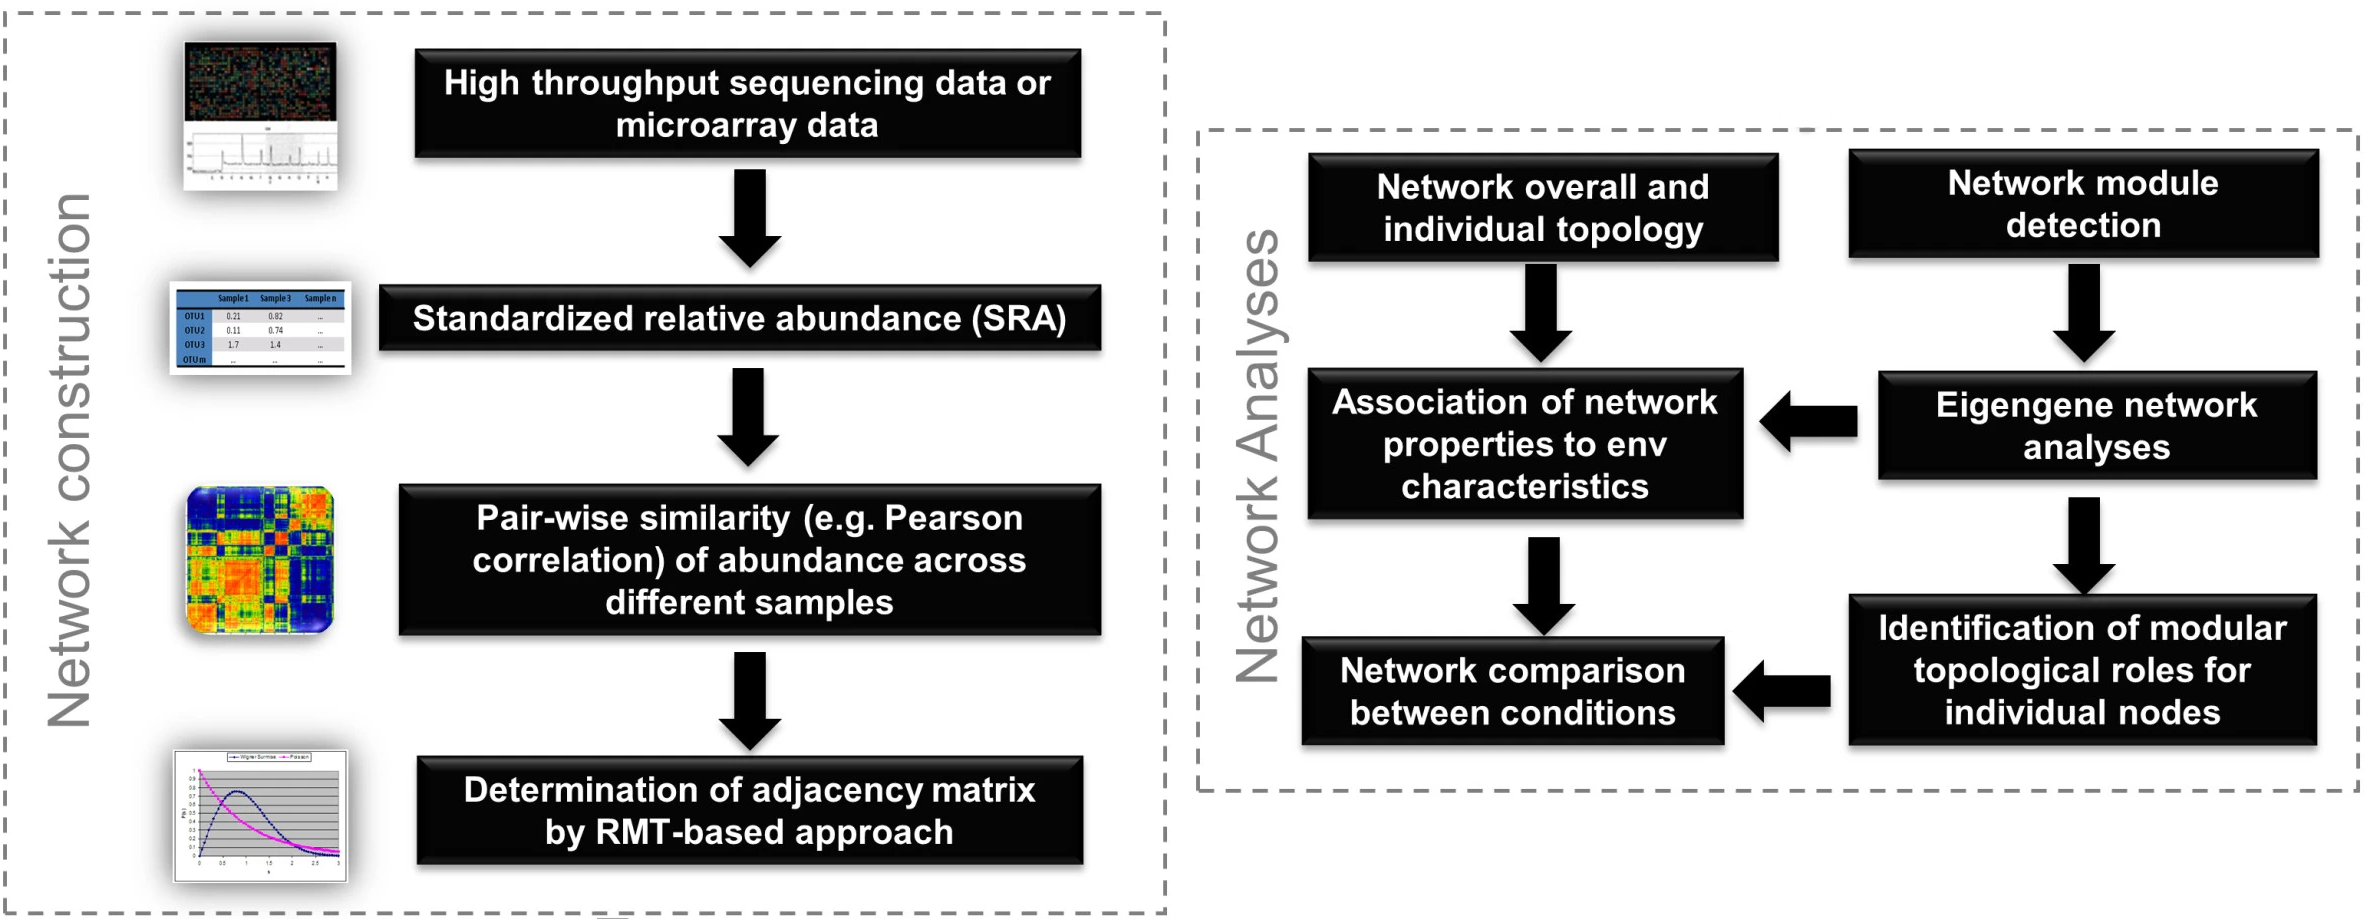
\includegraphics[width=1\textwidth]{Overview_of_the_Random_Matrix_Theory__RMT_-based_molecular_ecological_network_analysis_horizontal} % Path to your image file
    \caption{Overview of the Random Matrix Theory (RMT)-based molecular ecological network analysis\cite{deng_molecular_2012}}
    \label{fig:Overview_of_the_Random_Matrix_Theory__RMT_-based_molecular_ecological_network_analysis}
\end{figure}

The first phase(\autoref{fig:Overview_of_the_Random_Matrix_Theory__RMT_-based_molecular_ecological_network_analysis}) is network construction, which involves data collection of data then its transformation or standardization to normalize, calculation of pairwise similarity matrices, and the determination of the adjacency matrix using Random Matrix Theory.
The RMT-based approach is crucial for constructing an accurate network by defining an objective thresholds, resulting in an undirected network graph.

The second phase(\autoref{fig:Overview_of_the_Random_Matrix_Theory__RMT_-based_molecular_ecological_network_analysis}) is network analysis, which includes network topology characterization to evaluate the overall structure and properties of the network and the module detection to identify groups of tightly connected nodes known as modules.
Then a module-based eigengene analysis to understand underlying patterns and functions, and the identification of modular roles to determine the importance and function of nodes within modules.
An eigengene is a concept used in computational biology and bioinformatics to summarize the expression profiles of a group of co-expressed genes within a gene expression dataset.
Specifically, in the context of Weighted Gene Correlation Network Analysis (WGCNA), eigengenes serve as representative profiles for modules (clusters) of highly correlated genes or weighted combination of gene expressions that captures significant variation.
Additionally, eigengene network analysis explores higher-order organizational structures within the network, and associations between network properties and environmental characteristics are established to understand environmental influences.
Finally, comparative analysis evaluates network differences under varying conditions to assess how environmental changes affect network structure and interactions.
\\\\
Collectively, these methods enable researchers to uncover the complex interactions within microbial ecosystems, identify key functional populations at the OTU level, and understand how environmental factors influence these networks.

\newpage
\subsection{Determination Of The Adjacency Matrix Using \mbox{Random} Matrix Theory}\label{subsec:determination-of-the-adjacency-matrix-using-random-matrix-theory}

RMT is used in MENA as a way to automatically identify thresholds for network construction(\autoref{fig:Process_of_random_matrix_theory-based_approach_for_automatically_detecting_threshold_to_construct_molecular_ecological_networks}).
It is able to do that by examining the statistical properties of matrices derived from high-throughput ecological data.

\begin{figure}[H]
    \centering
    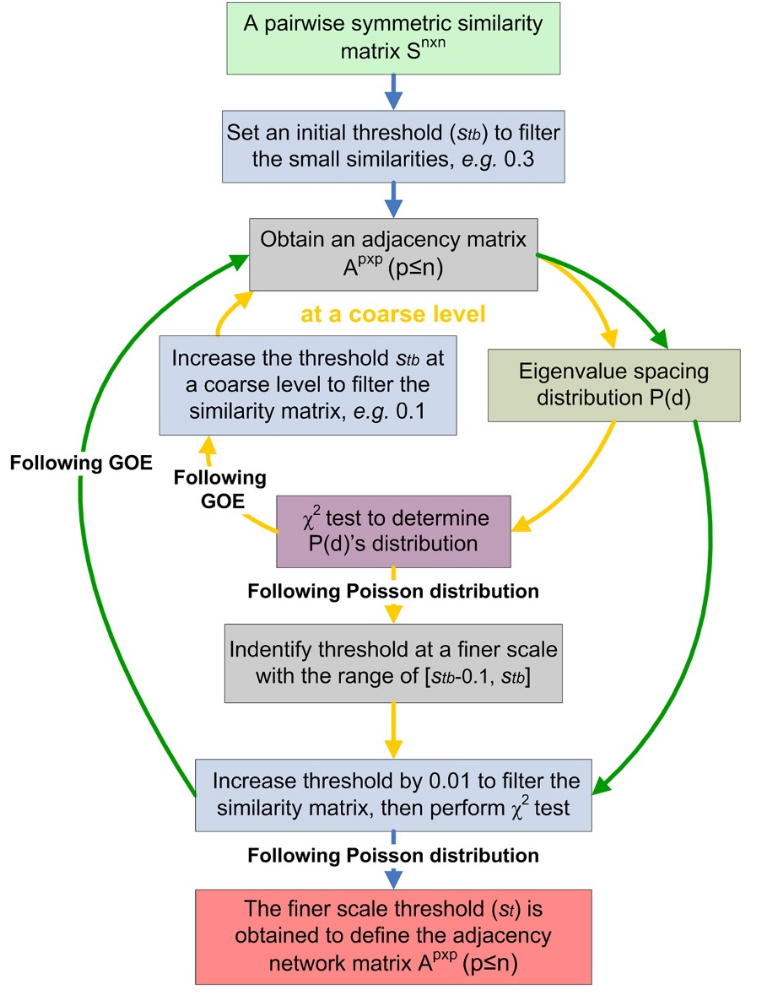
\includegraphics[width=0.72\textwidth]{Process of random matrix theory-based approach for automatically detecting threshold to construct molecular ecological networks} % Path to your image file
    \caption{Process of random matrix theory-based approach for automatically detecting a threshold to construct molecular ecological networks\cite{deng_molecular_2012}}
    \label{fig:Process_of_random_matrix_theory-based_approach_for_automatically_detecting_threshold_to_construct_molecular_ecological_networks}
\end{figure}

At first, the Pearson correlation matrix $R^{nxn}$ has to be computed using the standardized relative abundances of OTUs $X^{nxm}$, where $n$ is the number of distinct OTUs and $m$ is the number of samples.
This matrix $R^{nxn}$ is rapidly transformed into a similarity matrix $S^{nxn}$ by just taking the absolute values of $R^{nxn}$.
An adjacency matrix $A^{pxp}$, where p is the number of OTUs retained in the adjacency matrix with non-zero rows or columns, is then defined according to a threshold $s_{tb}$ set at first at 0.3.
The adjacency $a_{ij}$ between the i-th and j-th OTU is defined by thresholding the OTU abundance similarity:
\[a_{ij} =
\begin{cases}
s_{ij} & \text{if } s_{ij} \geq s_t, \\
0 & \text{if } s_{ij} < s_t.
\end{cases}\]
\\\\
\noindent The eigenvalues $\lambda_i$ of the adjacency matrix $A^{pxp}$ are then calculated.
Since it $A^{pxp}$ is a symmetric matrix, p eigenvalues can be obtained.
To test the Nearest Neighbor Spacing Distributions (NNDS), the eigenvalues are ordered as $\lambda_1 \leq \lambda_2 \leq \ldots \leq \lambda_p$.
To unfold the eigenvalues, $\lambda_i$ is replaced by $e_i = N_{av}(\lambda_i)$ where $N_{av}$ is the continuous density of eigenvalues.
The continuous density $N_{av}$ can be obtained either by fitting the original integrated density to a cubic spline or by calculating the local average.
\\\\
The NNDS $P(s)$ is then calculated by taking the absolute value of the difference between consecutive eigenvalues.
This defines the probability density of unfolded eigenvalues spacing.
For the completely uncorrelated eigenvalues, P(d) follows Poisson statistic, and it can be expressed by, $P(s)=e^{-d}$ and the correlated eigenvalues, P(d) closely follow Wigner-Dyson distribution of the GOE statistics, and it can be expressed by $P(s) \approx \frac{\pi s}{2}e^{-\frac{\pi}{4}s^2}$(\autoref{fig:Wigner-Dyson_and_Poisson_distribution}).

\begin{figure}[H]
    \centering
    \includegraphics[width=1\textwidth]{Wigner’s surmise and Poisson} % Path to your image file
    \caption{Wigner-Dyson (blue) and Poisson (orange) distribution}
    \label{fig:Wigner-Dyson_and_Poisson_distribution}
\end{figure}

To determine whether the NNDS follows the Wigner-Dyson distribution or the Poisson distribution, the chi-squared test is used to fit it to the Poisson distribution.
By establishing the null hypothesis $H_0$ that $P(d)$ follows a Poisson distribution, the NNSD is tested to see if it conforms to this distribution.
If the NNSD does follow a Poisson distribution, then 0.1 is subtracted to the current threshold and then increases the threshold incrementally by 0.01 instead of 0.1.
This is tested by a $\chi^2$ defined like:
\[\chi^2=\sum \frac{(d_i-E(d_i))^2}{E(d_i)}\]
With $d_i$ the observed nearest neighbor spacing and $E(d_i)$ the expected nearest neighbor spacing from Poisson distribution.

\noindent After determining the final threshold value $s_t$ at a finer scale, an adjacency matrix is constructed by retaining all OTUs with abundance similarity values exceeding the defined threshold.
Therefore, the final adjacency matrix will be defined like $A^{pxp}=[a_{ij}]$ is:

\[a_{ij} =
\begin{cases}
1 & \text{if } s_{ij} \geq s_t, \\
0 & \text{if } s_{ij} < s_t.
\end{cases}\]
\\\\
\noindent Here is a Python code snippet that demonstrates the process of determining the adjacency matrix using RMT.
It is assumed that, and the eigenvalues $\lambda_i$ of the adjacency matrix $A^{p \times p}$ are available.
\\\\
\begin{figure}[H] % H forces the figure to appear exactly here
\centering
\begin{lstlisting}[
    label={lst:pythoncode},
    language=Python,
    basicstyle=\fontsize{9pt}{13pt}\ttfamily, % Adjust font size and line spacing
]
import numpy as np
from scipy.interpolate import UnivariateSpline
from scipy.stats import chi2
np.random.seed(74)

# Generate sample eigenvalues for testing
N = 10000
lambdas = np.random.normal(loc=0, scale=1, size=N)
lambdas.sort()

N_lambda = np.arange(1, N + 1)  # Integrated density N(lambda_i) = i

# Create the spline with smoothing
spline = UnivariateSpline(lambdas, N_lambda, s=N, k=3)

# Compute N_av(lambda_i)
e_i = spline(lambdas)

# Compute the NNDS
spacings = abs(np.diff(e_i))

# Compute the pdf of spacings
p_s, bin_edges = np.histogram(spacings, bins=50, density=True)
s = 0.5 * (bin_edges[:-1] + bin_edges[1:])

# Compute the chi-squared statistic
poisson = np.exp(-s)
chi2_stat = np.sum((p_s - poisson) ** 2 / poisson)
if chi2_stat <= chi2.ppf(0.95, 50 - 1): print("H0 is not rejected")
else: print("H0 is rejected")
\end{lstlisting}
\caption{Python code for determining the threshold for the adjacency matrix using RMT}
\label{fig:pythoncode}
\end{figure}

This code snippet~(\autoref{fig:pythoncode}) demonstrates hwo easy the process of determining the adjacency matrix using RMT can be.
From this, it is concluded that "0.32 $\leq$ 6.63 so H0 is not rejected" indicating that it is the right threshold because the NNSD is consistent with the Poisson distribution~(\autoref{fig:Histogram_of_spacings_and_expected_spacings}).
Indeed, since the eigenvalues are generated using a normal distribution, these eigenvalues are uncorrelated by design.
This is the best case scenario, real data rarely behaves like this.
This simplicity mixed with the robustness of determining a threshold with RMT makes this method very elegant.

\begin{figure}[H]
    \centering
    \includegraphics[width=1\textwidth]{Wigner’s surmise and Poisson fitting P(s)} % Path to your image file
    \caption{Histogram of spacings compared to the expected spacings (Poisson distribution) and the Wigner-Dyson distribution}
    \label{fig:Histogram_of_spacings_and_expected_spacings}
\end{figure}

\noindent Thus, the adjacency matrix is constructed using the threshold $s_t$ determined by RMT, ensuring that the network is constructed objectively and consistently.

\subsection{Comparison To Legacy Network Methods And Robustness}\label{subsec:comparison-to-legacy-network-methods-and-robustness}

Both methodologies aim to understand relationships among biological entities, but they differ in principles, computational frameworks, and applications.
MENA uses advanced statistical tools like RMT to create robust, automated ecological networks.
In contrast, Legacy Co-Expression Network Analysis (LCNA) typically depends on co-expression thresholds to identify gene modules.
The table below compares these approaches, outlining their features, strengths, and limitations.
This comparison helps researchers choose the right method based on their research goals and data.

\begin{table}[H]
\centering
\renewcommand{\arraystretch}{1.5} % Adjusts row height
\begin{tabularx}{\textwidth}{@{}p{0.25\textwidth}X X@{}}
\toprule
\textbf{Feature} & \textbf{MENA} & \textbf{LCNA} \\
\midrule
\textbf{Network Construction Method} &
Uses Random Matrix Theory (RMT) for threshold determination, avoiding arbitrary cutoffs\cite{deng_molecular_2012} &
Relies on soft/hard thresholding or predefined cutoff values, which are subjective\cite{butte_discovering_2000} \\

\textbf{Robustness to Noise} &
Highly robust due to the RMT-based framework\cite{deng_molecular_2012} &
Sensitive to threshold selection and noise in data\cite{deng_molecular_2012} \\

\textbf{Topology Characteristics} &
Identifies scale-free, small-world, and modular networks\cite{deng_molecular_2012} &
Focuses on identifying clusters but may miss modular hierarchy\cite{horvath_analysis_2006} \\

\textbf{Key Applications} &
Analyzing ecological and environmental interactions, such as microbial community responses\cite{deng_molecular_2012} &
Studying biological processes like disease susceptibility and functional gene modules\cite{butte_discovering_2000,zhang_general_2005} \\

\textbf{Threshold Determination} &
Automated through RMT to ensure consistency\cite{deng_molecular_2012} &
Arbitrary or empirically determined, leading to biases\cite{deng_molecular_2012} \\

\textbf{Integration with Functional Data} &
Facilitates module-based eigengene analysis for deeper insights\cite{deng_molecular_2012} &
Limited integration with functional data without additional preprocessing\cite{horvath_analysis_2006} \\

\textbf{Software Availability} &
Supported by tools online for streamlined analysis\cite{deng_molecular_2012} &
Requires multiple tools or manual pipelines, such as clustering and visualization packages\cite{deng_molecular_2012} \\
\bottomrule
\end{tabularx}
\caption{Comparison of MENA and Legacy Co-Expression Network Analysis Methods}
\label{tab:mena_vs_lcna}
\end{table}

With this table(\autoref{tab:mena_vs_lcna}), it is clear that MENA and LCNA have distinct advantages and limitations.
MENA uses RMT for automated thresholding, reducing subjective bias.
In high-throughput ecological studies where noise is a concern, this makes it a great choice.
Because of the need for a better understanding of the network topology and environmental interactions, new methods like MENA are essential.
The analyses on modularity and eigengene is a fantastic help in the comprehension of the molecular ecological networks.
However, it keeps the co-expression network analysis downsides such as the reliance on simplistic correlation metrics.

\noindent In contrast, some LCNA are simpler of use, making it more accessible when computational resources or specialized tools are limited.
In spite of this, the subjectivity with the threshold selection and noise can result in inconsistencies in network structure.
LCNA’s adaptability to diverse datasets has a solid role as a foundational approach in network biology.
\\\\
Both approaches have distinct roles.
Complex ecological data analysis is where MENA shine, while LCNA offers a practical entry point for studying gene expression in simpler contexts.
Future developments may integrate MENA’s robustness with the different LCNA’s strong points like accessibility and the inclusion of complexe data.
Researchers should choose the method that best fits their dataset, goals, and computational expertise.



\section{Discussion}\label{sec:discussion}
The evolution of gene network analysis methods, as explored in this work, demonstrates a significant trajectory of progress in both theoretical and practical frameworks for understanding complex biological systems.
From the foundational applications of graph theory to modern techniques incorporating Random Matrix Theory (RMT), this journey reflects the increasing demand for precision, robustness, and interpretability in genomic data analysis.


\subsection*{Key Findings}

One of the primary conclusions drawn from this study is the clear advantage of integrating advanced mathematical frameworks like RMT into MENA\@.
Traditional approaches, such as equation-based networks or Bayesian methods, while insightful, often suffer from limitations related to subjective thresholding, sensitivity to noise, or scalability issues.
RMT-based methods provide an objective, systematic mechanism for threshold determination, enhancing the reliability of network construction and reducing biases that might otherwise skew biological interpretations.
\\\\
\noindent The application of MENA and its comparison to LCNA highlight their respective strengths and limitations.
LCNA remains a practical entry point for studying simpler gene interactions due to its accessibility and longstanding use in biology.
However, MENA’s advanced features, such as eigengene analysis and robust modularity detection, position it as a superior choice for analyzing complex ecological or environmental datasets where noise and dynamic interactions are prevalent.

\subsection*{Implications for Future Research}

This study underscores the necessity of continued innovation in network analysis methodologies.
While RMT-based techniques address many limitations of traditional approaches, challenges remain, particularly in terms of computational demands and the integration of multi-omics data.
Future research should explore hybrid methodologies that combine the robustness of RMT with the simplicity and computational efficiency of legacy methods.
Additionally, the increasing availability of high-throughput data presents an opportunity to refine these approaches, ensuring they remain scalable and adaptable to diverse biological contexts.
\\\\
\noindent Another avenue for advancement lies in the exploration of temporal dynamics within gene networks.
Current methods predominantly focus on static representations, but the inclusion of temporal data could provide deeper insights into regulatory mechanisms and adaptive responses.
This would require further development of both mathematical models and computational tools capable of handling dynamic, high-dimensional datasets.
\\\\
Furthermore, MENAP is, for now, only accessible online, making it difficult for researchers to customize or extend its functionalities or just verify the code.
Future developments should focus on creating a user-friendly, open source version of MENAP that allows for greater flexibility and transparency in network analysis.
Broader adoption of the pipeline would be facilitated, and collaboration across research communities would be encouraged, ultimately advancing the understanding of gene networks.
Having a local version of MENAP is expected to make researchers who were not comfortable sending their data to the online version feel more at ease using it.

\subsection*{Broader Impact}

The advancements discussed in this work have implications beyond genomics, extending to fields such as ecology, systems biology, and even financial modeling, where the principles of RMT have found application.
A paradigm shift in the approach to biological data is represented by the integration of RMT into gene network analysis, emphasizing the importance of robustness, objectivity, and scalability in network construction.
The beauty of RMT lies in its origins from an entirely different field and its successful application to genomics, exemplifying how interdisciplinary research can drive groundbreaking discoveries.
\\\\
\noindent This bibliography serves as a testimony to the power of interdisciplinary collaboration and the potential for transformative innovation when diverse fields converge.
It is also suggested that an attempt should be made to apply RMT to other domains of biology.

\section{Conclusion}\label{sec:conclusion}
In conclusion, the integration of RMT into gene network analysis represents a pivotal step toward more robust and meaningful biological interpretations.
By addressing the limitations of traditional methods and embracing the complexity of biological systems, RMT-based approaches pave the way for a deeper understanding of gene interactions and their implications in molecular ecology.
Continued collaboration across disciplines will be essential to harness the full potential of these methodologies, driving innovation and discovery in the years to come.

\noindent The innovations that led to the creation of MENA should serve as great motivation.
A motivation that helps researchers continue to push the boundaries of what is possible in gene network analysis and for exploring the application of RMT to other domains of biology.
For example, when used in cellular biology, RMT provides a great tool for analyzing the inherent noise and sparsity in single-cell genomic datasets.
It has been applied on a model based on data of random noise, sparsity-induced artifacts, and genuine biological signals that RMT helped disentangle these components effectively.
Ultimately, RMT-based methods facilitate deeper insights into complex biological systems, and help researchers to enhance the reliability and the precision of their findings.


\newpage
\addcontentsline{toc}{section}{References}
\printbibliography

\newpage

\section*{Abstract}\label{sec:abstract}
Gene network analysis plays an important role in the understanding of biological systems, including development, disease, and ecology.
This study reviews the development of gene network analysis methods, comparing traditional approaches like equation-based and Bayesian methods with newer techniques based on Random Matrix Theory (RMT). Traditional methods often struggle with scalability, sensitivity to noise, and subjective thresholding.
In contrast, RMT offers a systematic and reliable way to determine thresholds automatically.
Its integration into the Molecular Ecological Network Analysis pipeline strengthens gene network construction by reducing noise, minimizing bias, and increasing robustness.
This approach improves the understanding of system modularity and dynamics, addressing the limitations of older methods.
This bibliography puts in light RMT's potential to transform gene network analysis and expand its applications in biology and ecology.


\vfill % Push content to the bottom

\section*{Keywords}
\noindent Gene Network, Random Matrix Theory, Molecular Ecology, Network Analysis
\thispagestyle{firstpagestyle}
\end{document}